% Created by tikzDevice version 0.12 on 2019-07-15 13:07:42
% !TEX encoding = UTF-8 Unicode
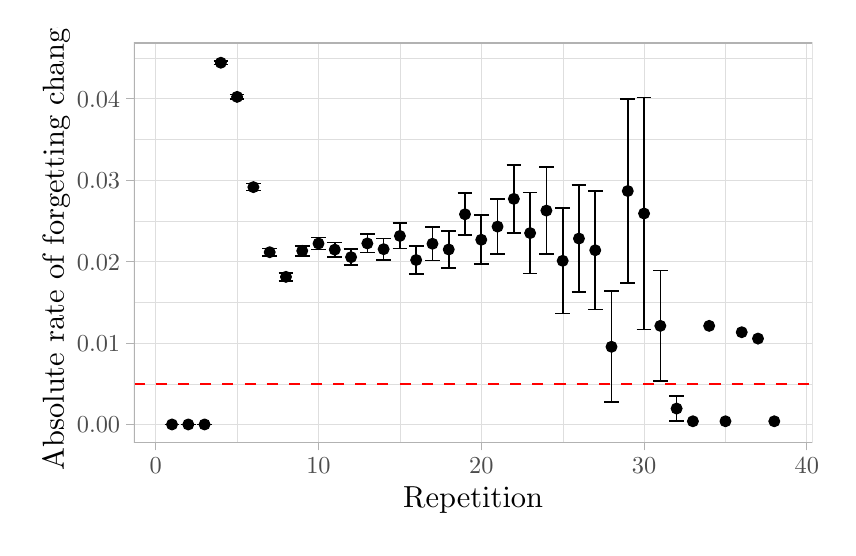
\begin{tikzpicture}[x=1pt,y=1pt]
\definecolor{fillColor}{RGB}{255,255,255}
\path[use as bounding box,fill=fillColor,fill opacity=0.00] (0,0) rectangle (289.08,180.67);
\begin{scope}
\path[clip] (  0.00,  0.00) rectangle (289.08,180.67);
\definecolor{drawColor}{RGB}{255,255,255}
\definecolor{fillColor}{RGB}{255,255,255}

\path[draw=drawColor,line width= 0.6pt,line join=round,line cap=round,fill=fillColor] (  0.00, -0.00) rectangle (289.08,180.67);
\end{scope}
\begin{scope}
\path[clip] ( 38.36, 30.72) rectangle (283.58,175.17);
\definecolor{fillColor}{RGB}{255,255,255}

\path[fill=fillColor] ( 38.36, 30.72) rectangle (283.58,175.17);
\definecolor{drawColor}{gray}{0.87}

\path[draw=drawColor,line width= 0.1pt,line join=round] ( 38.36, 52.00) --
	(283.58, 52.00);

\path[draw=drawColor,line width= 0.1pt,line join=round] ( 38.36, 81.42) --
	(283.58, 81.42);

\path[draw=drawColor,line width= 0.1pt,line join=round] ( 38.36,110.84) --
	(283.58,110.84);

\path[draw=drawColor,line width= 0.1pt,line join=round] ( 38.36,140.26) --
	(283.58,140.26);

\path[draw=drawColor,line width= 0.1pt,line join=round] ( 38.36,169.68) --
	(283.58,169.68);

\path[draw=drawColor,line width= 0.1pt,line join=round] ( 75.68, 30.72) --
	( 75.68,175.17);

\path[draw=drawColor,line width= 0.1pt,line join=round] (134.50, 30.72) --
	(134.50,175.17);

\path[draw=drawColor,line width= 0.1pt,line join=round] (193.32, 30.72) --
	(193.32,175.17);

\path[draw=drawColor,line width= 0.1pt,line join=round] (252.14, 30.72) --
	(252.14,175.17);

\path[draw=drawColor,line width= 0.3pt,line join=round] ( 38.36, 37.29) --
	(283.58, 37.29);

\path[draw=drawColor,line width= 0.3pt,line join=round] ( 38.36, 66.71) --
	(283.58, 66.71);

\path[draw=drawColor,line width= 0.3pt,line join=round] ( 38.36, 96.13) --
	(283.58, 96.13);

\path[draw=drawColor,line width= 0.3pt,line join=round] ( 38.36,125.55) --
	(283.58,125.55);

\path[draw=drawColor,line width= 0.3pt,line join=round] ( 38.36,154.97) --
	(283.58,154.97);

\path[draw=drawColor,line width= 0.3pt,line join=round] ( 46.27, 30.72) --
	( 46.27,175.17);

\path[draw=drawColor,line width= 0.3pt,line join=round] (105.09, 30.72) --
	(105.09,175.17);

\path[draw=drawColor,line width= 0.3pt,line join=round] (163.91, 30.72) --
	(163.91,175.17);

\path[draw=drawColor,line width= 0.3pt,line join=round] (222.73, 30.72) --
	(222.73,175.17);

\path[draw=drawColor,line width= 0.3pt,line join=round] (281.55, 30.72) --
	(281.55,175.17);
\definecolor{drawColor}{RGB}{0,0,0}
\definecolor{fillColor}{RGB}{0,0,0}

\path[draw=drawColor,line width= 0.4pt,line join=round,line cap=round,fill=fillColor] ( 52.15, 37.29) circle (  1.96);

\path[draw=drawColor,line width= 0.4pt,line join=round,line cap=round,fill=fillColor] ( 58.04, 37.29) circle (  1.96);

\path[draw=drawColor,line width= 0.4pt,line join=round,line cap=round,fill=fillColor] ( 63.92, 37.29) circle (  1.96);

\path[draw=drawColor,line width= 0.4pt,line join=round,line cap=round,fill=fillColor] ( 69.80,168.00) circle (  1.96);

\path[draw=drawColor,line width= 0.4pt,line join=round,line cap=round,fill=fillColor] ( 75.68,155.66) circle (  1.96);

\path[draw=drawColor,line width= 0.4pt,line join=round,line cap=round,fill=fillColor] ( 81.56,123.05) circle (  1.96);

\path[draw=drawColor,line width= 0.4pt,line join=round,line cap=round,fill=fillColor] ( 87.45, 99.53) circle (  1.96);

\path[draw=drawColor,line width= 0.4pt,line join=round,line cap=round,fill=fillColor] ( 93.33, 90.63) circle (  1.96);

\path[draw=drawColor,line width= 0.4pt,line join=round,line cap=round,fill=fillColor] ( 99.21,100.03) circle (  1.96);

\path[draw=drawColor,line width= 0.4pt,line join=round,line cap=round,fill=fillColor] (105.09,102.67) circle (  1.96);

\path[draw=drawColor,line width= 0.4pt,line join=round,line cap=round,fill=fillColor] (110.97,100.46) circle (  1.96);

\path[draw=drawColor,line width= 0.4pt,line join=round,line cap=round,fill=fillColor] (116.86, 97.75) circle (  1.96);

\path[draw=drawColor,line width= 0.4pt,line join=round,line cap=round,fill=fillColor] (122.74,102.71) circle (  1.96);

\path[draw=drawColor,line width= 0.4pt,line join=round,line cap=round,fill=fillColor] (128.62,100.63) circle (  1.96);

\path[draw=drawColor,line width= 0.4pt,line join=round,line cap=round,fill=fillColor] (134.50,105.41) circle (  1.96);

\path[draw=drawColor,line width= 0.4pt,line join=round,line cap=round,fill=fillColor] (140.38, 96.71) circle (  1.96);

\path[draw=drawColor,line width= 0.4pt,line join=round,line cap=round,fill=fillColor] (146.27,102.59) circle (  1.96);

\path[draw=drawColor,line width= 0.4pt,line join=round,line cap=round,fill=fillColor] (152.15,100.52) circle (  1.96);

\path[draw=drawColor,line width= 0.4pt,line join=round,line cap=round,fill=fillColor] (158.03,113.24) circle (  1.96);

\path[draw=drawColor,line width= 0.4pt,line join=round,line cap=round,fill=fillColor] (163.91,104.03) circle (  1.96);

\path[draw=drawColor,line width= 0.4pt,line join=round,line cap=round,fill=fillColor] (169.79,108.79) circle (  1.96);

\path[draw=drawColor,line width= 0.4pt,line join=round,line cap=round,fill=fillColor] (175.68,118.80) circle (  1.96);

\path[draw=drawColor,line width= 0.4pt,line join=round,line cap=round,fill=fillColor] (181.56,106.45) circle (  1.96);

\path[draw=drawColor,line width= 0.4pt,line join=round,line cap=round,fill=fillColor] (187.44,114.57) circle (  1.96);

\path[draw=drawColor,line width= 0.4pt,line join=round,line cap=round,fill=fillColor] (193.32, 96.43) circle (  1.96);

\path[draw=drawColor,line width= 0.4pt,line join=round,line cap=round,fill=fillColor] (199.20,104.47) circle (  1.96);

\path[draw=drawColor,line width= 0.4pt,line join=round,line cap=round,fill=fillColor] (205.09,100.24) circle (  1.96);

\path[draw=drawColor,line width= 0.4pt,line join=round,line cap=round,fill=fillColor] (210.97, 65.36) circle (  1.96);

\path[draw=drawColor,line width= 0.4pt,line join=round,line cap=round,fill=fillColor] (216.85,121.64) circle (  1.96);

\path[draw=drawColor,line width= 0.4pt,line join=round,line cap=round,fill=fillColor] (222.73,113.52) circle (  1.96);

\path[draw=drawColor,line width= 0.4pt,line join=round,line cap=round,fill=fillColor] (228.61, 72.92) circle (  1.96);

\path[draw=drawColor,line width= 0.4pt,line join=round,line cap=round,fill=fillColor] (234.49, 43.04) circle (  1.96);

\path[draw=drawColor,line width= 0.4pt,line join=round,line cap=round,fill=fillColor] (240.38, 38.44) circle (  1.96);

\path[draw=drawColor,line width= 0.4pt,line join=round,line cap=round,fill=fillColor] (246.26, 72.92) circle (  1.96);

\path[draw=drawColor,line width= 0.4pt,line join=round,line cap=round,fill=fillColor] (252.14, 38.44) circle (  1.96);

\path[draw=drawColor,line width= 0.4pt,line join=round,line cap=round,fill=fillColor] (258.02, 70.62) circle (  1.96);

\path[draw=drawColor,line width= 0.4pt,line join=round,line cap=round,fill=fillColor] (263.90, 68.32) circle (  1.96);

\path[draw=drawColor,line width= 0.4pt,line join=round,line cap=round,fill=fillColor] (269.79, 38.44) circle (  1.96);

\path[draw=drawColor,line width= 0.6pt,line join=round] ( 49.51, 37.29) --
	( 54.80, 37.29);

\path[draw=drawColor,line width= 0.6pt,line join=round] ( 52.15, 37.29) --
	( 52.15, 37.29);

\path[draw=drawColor,line width= 0.6pt,line join=round] ( 49.51, 37.29) --
	( 54.80, 37.29);

\path[draw=drawColor,line width= 0.6pt,line join=round] ( 55.39, 37.29) --
	( 60.68, 37.29);

\path[draw=drawColor,line width= 0.6pt,line join=round] ( 58.04, 37.29) --
	( 58.04, 37.29);

\path[draw=drawColor,line width= 0.6pt,line join=round] ( 55.39, 37.29) --
	( 60.68, 37.29);

\path[draw=drawColor,line width= 0.6pt,line join=round] ( 61.27, 37.29) --
	( 66.56, 37.29);

\path[draw=drawColor,line width= 0.6pt,line join=round] ( 63.92, 37.29) --
	( 63.92, 37.29);

\path[draw=drawColor,line width= 0.6pt,line join=round] ( 61.27, 37.29) --
	( 66.56, 37.29);

\path[draw=drawColor,line width= 0.6pt,line join=round] ( 67.15,168.61) --
	( 72.45,168.61);

\path[draw=drawColor,line width= 0.6pt,line join=round] ( 69.80,168.61) --
	( 69.80,167.39);

\path[draw=drawColor,line width= 0.6pt,line join=round] ( 67.15,167.39) --
	( 72.45,167.39);

\path[draw=drawColor,line width= 0.6pt,line join=round] ( 73.03,156.54) --
	( 78.33,156.54);

\path[draw=drawColor,line width= 0.6pt,line join=round] ( 75.68,156.54) --
	( 75.68,154.79);

\path[draw=drawColor,line width= 0.6pt,line join=round] ( 73.03,154.79) --
	( 78.33,154.79);

\path[draw=drawColor,line width= 0.6pt,line join=round] ( 78.92,124.32) --
	( 84.21,124.32);

\path[draw=drawColor,line width= 0.6pt,line join=round] ( 81.56,124.32) --
	( 81.56,121.78);

\path[draw=drawColor,line width= 0.6pt,line join=round] ( 78.92,121.78) --
	( 84.21,121.78);

\path[draw=drawColor,line width= 0.6pt,line join=round] ( 84.80,100.90) --
	( 90.09,100.90);

\path[draw=drawColor,line width= 0.6pt,line join=round] ( 87.45,100.90) --
	( 87.45, 98.17);

\path[draw=drawColor,line width= 0.6pt,line join=round] ( 84.80, 98.17) --
	( 90.09, 98.17);

\path[draw=drawColor,line width= 0.6pt,line join=round] ( 90.68, 92.12) --
	( 95.97, 92.12);

\path[draw=drawColor,line width= 0.6pt,line join=round] ( 93.33, 92.12) --
	( 93.33, 89.13);

\path[draw=drawColor,line width= 0.6pt,line join=round] ( 90.68, 89.13) --
	( 95.97, 89.13);

\path[draw=drawColor,line width= 0.6pt,line join=round] ( 96.56,101.82) --
	(101.86,101.82);

\path[draw=drawColor,line width= 0.6pt,line join=round] ( 99.21,101.82) --
	( 99.21, 98.24);

\path[draw=drawColor,line width= 0.6pt,line join=round] ( 96.56, 98.24) --
	(101.86, 98.24);

\path[draw=drawColor,line width= 0.6pt,line join=round] (102.44,104.84) --
	(107.74,104.84);

\path[draw=drawColor,line width= 0.6pt,line join=round] (105.09,104.84) --
	(105.09,100.49);

\path[draw=drawColor,line width= 0.6pt,line join=round] (102.44,100.49) --
	(107.74,100.49);

\path[draw=drawColor,line width= 0.6pt,line join=round] (108.33,103.01) --
	(113.62,103.01);

\path[draw=drawColor,line width= 0.6pt,line join=round] (110.97,103.01) --
	(110.97, 97.90);

\path[draw=drawColor,line width= 0.6pt,line join=round] (108.33, 97.90) --
	(113.62, 97.90);

\path[draw=drawColor,line width= 0.6pt,line join=round] (114.21,100.70) --
	(119.50,100.70);

\path[draw=drawColor,line width= 0.6pt,line join=round] (116.86,100.70) --
	(116.86, 94.80);

\path[draw=drawColor,line width= 0.6pt,line join=round] (114.21, 94.80) --
	(119.50, 94.80);

\path[draw=drawColor,line width= 0.6pt,line join=round] (120.09,106.05) --
	(125.38,106.05);

\path[draw=drawColor,line width= 0.6pt,line join=round] (122.74,106.05) --
	(122.74, 99.37);

\path[draw=drawColor,line width= 0.6pt,line join=round] (120.09, 99.37) --
	(125.38, 99.37);

\path[draw=drawColor,line width= 0.6pt,line join=round] (125.97,104.51) --
	(131.27,104.51);

\path[draw=drawColor,line width= 0.6pt,line join=round] (128.62,104.51) --
	(128.62, 96.76);

\path[draw=drawColor,line width= 0.6pt,line join=round] (125.97, 96.76) --
	(131.27, 96.76);

\path[draw=drawColor,line width= 0.6pt,line join=round] (131.85,109.98) --
	(137.15,109.98);

\path[draw=drawColor,line width= 0.6pt,line join=round] (134.50,109.98) --
	(134.50,100.85);

\path[draw=drawColor,line width= 0.6pt,line join=round] (131.85,100.85) --
	(137.15,100.85);

\path[draw=drawColor,line width= 0.6pt,line join=round] (137.74,101.83) --
	(143.03,101.83);

\path[draw=drawColor,line width= 0.6pt,line join=round] (140.38,101.83) --
	(140.38, 91.60);

\path[draw=drawColor,line width= 0.6pt,line join=round] (137.74, 91.60) --
	(143.03, 91.60);

\path[draw=drawColor,line width= 0.6pt,line join=round] (143.62,108.60) --
	(148.91,108.60);

\path[draw=drawColor,line width= 0.6pt,line join=round] (146.27,108.60) --
	(146.27, 96.57);

\path[draw=drawColor,line width= 0.6pt,line join=round] (143.62, 96.57) --
	(148.91, 96.57);

\path[draw=drawColor,line width= 0.6pt,line join=round] (149.50,107.15) --
	(154.79,107.15);

\path[draw=drawColor,line width= 0.6pt,line join=round] (152.15,107.15) --
	(152.15, 93.89);

\path[draw=drawColor,line width= 0.6pt,line join=round] (149.50, 93.89) --
	(154.79, 93.89);

\path[draw=drawColor,line width= 0.6pt,line join=round] (155.38,120.84) --
	(160.68,120.84);

\path[draw=drawColor,line width= 0.6pt,line join=round] (158.03,120.84) --
	(158.03,105.64);

\path[draw=drawColor,line width= 0.6pt,line join=round] (155.38,105.64) --
	(160.68,105.64);

\path[draw=drawColor,line width= 0.6pt,line join=round] (161.26,112.86) --
	(166.56,112.86);

\path[draw=drawColor,line width= 0.6pt,line join=round] (163.91,112.86) --
	(163.91, 95.20);

\path[draw=drawColor,line width= 0.6pt,line join=round] (161.26, 95.20) --
	(166.56, 95.20);

\path[draw=drawColor,line width= 0.6pt,line join=round] (167.15,118.77) --
	(172.44,118.77);

\path[draw=drawColor,line width= 0.6pt,line join=round] (169.79,118.77) --
	(169.79, 98.82);

\path[draw=drawColor,line width= 0.6pt,line join=round] (167.15, 98.82) --
	(172.44, 98.82);

\path[draw=drawColor,line width= 0.6pt,line join=round] (173.03,131.02) --
	(178.32,131.02);

\path[draw=drawColor,line width= 0.6pt,line join=round] (175.68,131.02) --
	(175.68,106.59);

\path[draw=drawColor,line width= 0.6pt,line join=round] (173.03,106.59) --
	(178.32,106.59);

\path[draw=drawColor,line width= 0.6pt,line join=round] (178.91,121.10) --
	(184.20,121.10);

\path[draw=drawColor,line width= 0.6pt,line join=round] (181.56,121.10) --
	(181.56, 91.80);

\path[draw=drawColor,line width= 0.6pt,line join=round] (178.91, 91.80) --
	(184.20, 91.80);

\path[draw=drawColor,line width= 0.6pt,line join=round] (184.79,130.36) --
	(190.09,130.36);

\path[draw=drawColor,line width= 0.6pt,line join=round] (187.44,130.36) --
	(187.44, 98.78);

\path[draw=drawColor,line width= 0.6pt,line join=round] (184.79, 98.78) --
	(190.09, 98.78);

\path[draw=drawColor,line width= 0.6pt,line join=round] (190.67,115.43) --
	(195.97,115.43);

\path[draw=drawColor,line width= 0.6pt,line join=round] (193.32,115.43) --
	(193.32, 77.43);

\path[draw=drawColor,line width= 0.6pt,line join=round] (190.67, 77.43) --
	(195.97, 77.43);

\path[draw=drawColor,line width= 0.6pt,line join=round] (196.56,123.87) --
	(201.85,123.87);

\path[draw=drawColor,line width= 0.6pt,line join=round] (199.20,123.87) --
	(199.20, 85.06);

\path[draw=drawColor,line width= 0.6pt,line join=round] (196.56, 85.06) --
	(201.85, 85.06);

\path[draw=drawColor,line width= 0.6pt,line join=round] (202.44,121.64) --
	(207.73,121.64);

\path[draw=drawColor,line width= 0.6pt,line join=round] (205.09,121.64) --
	(205.09, 78.84);

\path[draw=drawColor,line width= 0.6pt,line join=round] (202.44, 78.84) --
	(207.73, 78.84);

\path[draw=drawColor,line width= 0.6pt,line join=round] (208.32, 85.40) --
	(213.61, 85.40);

\path[draw=drawColor,line width= 0.6pt,line join=round] (210.97, 85.40) --
	(210.97, 45.32);

\path[draw=drawColor,line width= 0.6pt,line join=round] (208.32, 45.32) --
	(213.61, 45.32);

\path[draw=drawColor,line width= 0.6pt,line join=round] (214.20,154.94) --
	(219.50,154.94);

\path[draw=drawColor,line width= 0.6pt,line join=round] (216.85,154.94) --
	(216.85, 88.34);

\path[draw=drawColor,line width= 0.6pt,line join=round] (214.20, 88.34) --
	(219.50, 88.34);

\path[draw=drawColor,line width= 0.6pt,line join=round] (220.08,155.40) --
	(225.38,155.40);

\path[draw=drawColor,line width= 0.6pt,line join=round] (222.73,155.40) --
	(222.73, 71.63);

\path[draw=drawColor,line width= 0.6pt,line join=round] (220.08, 71.63) --
	(225.38, 71.63);

\path[draw=drawColor,line width= 0.6pt,line join=round] (225.97, 92.95) --
	(231.26, 92.95);

\path[draw=drawColor,line width= 0.6pt,line join=round] (228.61, 92.95) --
	(228.61, 52.88);

\path[draw=drawColor,line width= 0.6pt,line join=round] (225.97, 52.88) --
	(231.26, 52.88);

\path[draw=drawColor,line width= 0.6pt,line join=round] (231.85, 47.63) --
	(237.14, 47.63);

\path[draw=drawColor,line width= 0.6pt,line join=round] (234.49, 47.63) --
	(234.49, 38.44);

\path[draw=drawColor,line width= 0.6pt,line join=round] (231.85, 38.44) --
	(237.14, 38.44);
\definecolor{drawColor}{RGB}{255,0,0}

\path[draw=drawColor,line width= 0.6pt,dash pattern=on 4pt off 4pt ,line join=round] ( 38.36, 51.88) -- (283.58, 51.88);
\definecolor{drawColor}{gray}{0.70}

\path[draw=drawColor,line width= 0.6pt,line join=round,line cap=round] ( 38.36, 30.72) rectangle (283.58,175.17);
\end{scope}
\begin{scope}
\path[clip] (  0.00,  0.00) rectangle (289.08,180.67);
\definecolor{drawColor}{gray}{0.30}

\node[text=drawColor,anchor=base east,inner sep=0pt, outer sep=0pt, scale=  0.88] at ( 33.41, 34.26) {0.00};

\node[text=drawColor,anchor=base east,inner sep=0pt, outer sep=0pt, scale=  0.88] at ( 33.41, 63.68) {0.01};

\node[text=drawColor,anchor=base east,inner sep=0pt, outer sep=0pt, scale=  0.88] at ( 33.41, 93.10) {0.02};

\node[text=drawColor,anchor=base east,inner sep=0pt, outer sep=0pt, scale=  0.88] at ( 33.41,122.52) {0.03};

\node[text=drawColor,anchor=base east,inner sep=0pt, outer sep=0pt, scale=  0.88] at ( 33.41,151.94) {0.04};
\end{scope}
\begin{scope}
\path[clip] (  0.00,  0.00) rectangle (289.08,180.67);
\definecolor{drawColor}{gray}{0.70}

\path[draw=drawColor,line width= 0.3pt,line join=round] ( 35.61, 37.29) --
	( 38.36, 37.29);

\path[draw=drawColor,line width= 0.3pt,line join=round] ( 35.61, 66.71) --
	( 38.36, 66.71);

\path[draw=drawColor,line width= 0.3pt,line join=round] ( 35.61, 96.13) --
	( 38.36, 96.13);

\path[draw=drawColor,line width= 0.3pt,line join=round] ( 35.61,125.55) --
	( 38.36,125.55);

\path[draw=drawColor,line width= 0.3pt,line join=round] ( 35.61,154.97) --
	( 38.36,154.97);
\end{scope}
\begin{scope}
\path[clip] (  0.00,  0.00) rectangle (289.08,180.67);
\definecolor{drawColor}{gray}{0.70}

\path[draw=drawColor,line width= 0.3pt,line join=round] ( 46.27, 27.97) --
	( 46.27, 30.72);

\path[draw=drawColor,line width= 0.3pt,line join=round] (105.09, 27.97) --
	(105.09, 30.72);

\path[draw=drawColor,line width= 0.3pt,line join=round] (163.91, 27.97) --
	(163.91, 30.72);

\path[draw=drawColor,line width= 0.3pt,line join=round] (222.73, 27.97) --
	(222.73, 30.72);

\path[draw=drawColor,line width= 0.3pt,line join=round] (281.55, 27.97) --
	(281.55, 30.72);
\end{scope}
\begin{scope}
\path[clip] (  0.00,  0.00) rectangle (289.08,180.67);
\definecolor{drawColor}{gray}{0.30}

\node[text=drawColor,anchor=base,inner sep=0pt, outer sep=0pt, scale=  0.88] at ( 46.27, 19.71) {0};

\node[text=drawColor,anchor=base,inner sep=0pt, outer sep=0pt, scale=  0.88] at (105.09, 19.71) {10};

\node[text=drawColor,anchor=base,inner sep=0pt, outer sep=0pt, scale=  0.88] at (163.91, 19.71) {20};

\node[text=drawColor,anchor=base,inner sep=0pt, outer sep=0pt, scale=  0.88] at (222.73, 19.71) {30};

\node[text=drawColor,anchor=base,inner sep=0pt, outer sep=0pt, scale=  0.88] at (281.55, 19.71) {40};
\end{scope}
\begin{scope}
\path[clip] (  0.00,  0.00) rectangle (289.08,180.67);
\definecolor{drawColor}{RGB}{0,0,0}

\node[text=drawColor,anchor=base,inner sep=0pt, outer sep=0pt, scale=  1.10] at (160.97,  7.44) {Repetition};
\end{scope}
\begin{scope}
\path[clip] (  0.00,  0.00) rectangle (289.08,180.67);
\definecolor{drawColor}{RGB}{0,0,0}

\node[text=drawColor,rotate= 90.00,anchor=base,inner sep=0pt, outer sep=0pt, scale=  1.10] at ( 13.08,102.95) {Absolute rate of forgetting change};
\end{scope}
\end{tikzpicture}
